\documentclass[11pt]{article}

\usepackage[margin=1in]{geometry}
\usepackage{graphicx}
\usepackage{booktabs}
\usepackage{array}
\usepackage{hyperref}
\usepackage{natbib}
\usepackage{xcolor}
\usepackage{float}

\graphicspath{{../output/}}

\hypersetup{
  colorlinks=true,
  linkcolor=blue,
  citecolor=blue,
  urlcolor=blue
}

\setlength{\parskip}{0.65em}
\setlength{\parindent}{0pt}

\title{\vspace{-1.3cm}Auditing a Text-Based Ranking Proxy in CHORUS:\\
A Reproducible Reward-Signal Reconstruction}
\author{Doris Wang\\
M.A. Computational Social Science, Economics Specialization\\
University of Chicago}
\date{May 2026}

\begin{document}
\maketitle

\begin{abstract}
This project audits how an AI research assistant can create ranking risk when a convenient textual signal is used as a proxy for intellectual value. CHORUS organizes a research lab through registry data and a directed hypergraph linking people, papers, topics, venues, projects, and computational resources. The recovered project folder contained the registry and hypergraph data, but not the original model artifacts needed to reproduce the earlier text-surprise and representation-contrast scores exactly. I therefore rebuild the audit as a transparent reconstruction rather than as a claimed recovery of the original scoring pipeline.

The rebuilt project creates a paper-level panel, defines clearly labeled proxy scores, and uses citation counts only as an external measure of uptake. The results suggest a directional selection problem. A text-focused ranking proxy can make papers with more complex titles more visible, while quieter papers with stronger external uptake may become easier to miss. The point is not that citations fully define scientific value, or that textual surprise is useless. The point is that an AI assistant should be audited for what it makes visible. In CHORUS, the object being ranked is a paper. In other AI-assisted decision environments, the object may be advice, actions, opportunities, or recommendations. In each case, the system does not only answer questions. It shapes what users notice, compare, and choose before they act.
\end{abstract}

\section{Research Question}

This project asks whether an AI assistant can create ranking risk when it uses
a convenient textual proxy to order research objects. The practical version of
the question is simple. If CHORUS is asked to surface papers that may deserve
attention, does a title based surprise proxy align with external evidence of
influence, or does it mainly surface papers whose titles look complex?

The conceptual question is broader. Many AI systems that support decision
making operate through ranking, recommendation, triage, or advice. They rarely
make a final decision by themselves. Instead, they reshape the information
environment in which people make decisions. The same audit logic applies
outside scientific retrieval. In any AI advice setting, the system compresses a
large choice set into a smaller set of visible options. A researcher may see a
ranked list of papers; a founder may see a short list of business suggestions;
a manager may see a ranked set of operational changes. In each case, the system
changes what becomes salient before the user acts.

This matters because a user may receive many possible recommendations and then
decide which one to implement. The relevant empirical question is not only
whether the model can generate plausible text. It is whether the ranking or
framing signal helps the user notice options that fit the user's actual
decision environment. If the compression is governed by an imperfect proxy, the
AI can make weak options more visible and useful options less visible.

\section{System Background}

CHORUS was built as a knowledge assistant for the University of Chicago
Knowledge Lab. The raw folder contains a registry of people, research topics,
projects, datasets, publications, and computational resources. It also contains
a hypergraph representation that connects people to documents, concepts,
venues, datasets, and other institutional objects. The system is meant to make
the lab searchable as a living research environment rather than as a static
folder of files.

The relevant design problem is the reward signal. A retrieval system has to
decide which objects deserve to be surfaced. One possible reward is text
surprise. A paper with a long title, multiple clauses, and unusual terms may
receive a high textual surprise score. That choice is tempting because text is
available and easy to process. It is also dangerous. A title can sound complex
without being scientifically central. A highly cited or institutionally
important paper can have a short title that does not announce its importance.

This creates a measurement problem. The system claims to reward intellectual
surprise, but it may partly reward title verbosity. If so, the problem is not
only noisy ranking. It is a directional ranking risk. A system can appear to be ranking carefully while still directing attention toward papers that are textually elaborate rather than substantively useful.

\section{Data Rebuild}

The recovered folder contained registry and hypergraph files, but not the model artifacts needed to reproduce the earlier scoring pipeline exactly. I reconstructed the audit from the available raw data. The rebuild uses the current recovered data snapshot. The recovered hypergraph contains 467 document nodes.
The registry contains 482 profile publication rows because some publications
appear in more than one profile before document consolidation.

\begin{table}[H]
\centering
\begin{tabular}{lrp{8.0cm}}
\toprule
Object & Count & Role in the rebuilt project \\
\midrule
People in registry & 71 & Used to attach names, roles, institutions, and topic labels to documents. \\
Profile publication rows & 482 & Used as the raw profile source before document consolidation. \\
Hypergraph document nodes & 467 & Used as the main paper level analysis sample. \\
Hypergraph edges & 594 & Used to recover links among publications, authors, topics, venues, and other objects. \\
\bottomrule
\end{tabular}
\caption{Raw CHORUS data used in the rebuilt audit.}
\end{table}

The rebuild creates one row per document node. Each row contains the title,
publication year, venue, citation count, title word count, linked lab authors,
author roles, topic count, and reconstructed scores. The code preserves both
sources of author information. The first source is the publication edge in the
hypergraph. The second source is the profile in which the publication appeared.
Keeping both sources visible matters because the registry is a constructed
research object, not a clean survey file. A reproducible audit should expose
that provenance rather than hide it.

\section{Measurement Strategy}

Two original model artifacts were absent from the recovered folder. The first
was the text surprise score, likely based on a language model perplexity
measure. The second was the representation contrast score, which measures how much a paper differs across representational views. Rather
than pretend those artifacts still existed, I rebuilt transparent proxy scores.

The text surprise proxy is based on title length and title syntax. This proxy is deliberately simple because the original language-model perplexity scores were not preserved. It should be read as a transparent stress test of a surface-text reward, not as a replacement for true perplexity. Long titles,
titles with colons, and titles with multiple clauses receive higher scores. This
is not meant to be a perfect language model measure. It is meant to represent
the kind of surface textual feature that a weak reward signal can overweight.

The representation contrast proxy uses information that is available before
looking at the outcome. It combines topic breadth, role diversity, venue
signal, and profile-link information. I intentionally keep this contrast proxy
separate from the title-based text-surprise score so that the quadrant
comparison is not mechanically generated by the same title-length measure.
Citation counts are held out as the audit outcome. This is important because
the project is not building a citation prediction model. The project is testing
whether a ranking signal that claims to capture scientific interest is aligned
with an external measure of uptake.

The analysis then creates three diagnostics.

\begin{enumerate}
  \item The title length diagnostic asks whether papers that look less
  surprising in title form are actually less influential.
  \item The quadrant diagnostic compares four regions of the score space:
  quiet high contrast papers, verbose high contrast papers, quiet low contrast
  papers, and verbose low contrast papers.
  \item The role diagnostic asks whether the signal reallocates attention
  across author groups. In this setting, the groups are based on lab role. In
  other settings, the same logic could be applied to founder experience,
  baseline firm performance, market type, geography, or digital skill.
\end{enumerate}

\section{Result 1. Title Verbosity Is a Risky Proxy}

\begin{figure}[H]
\centering
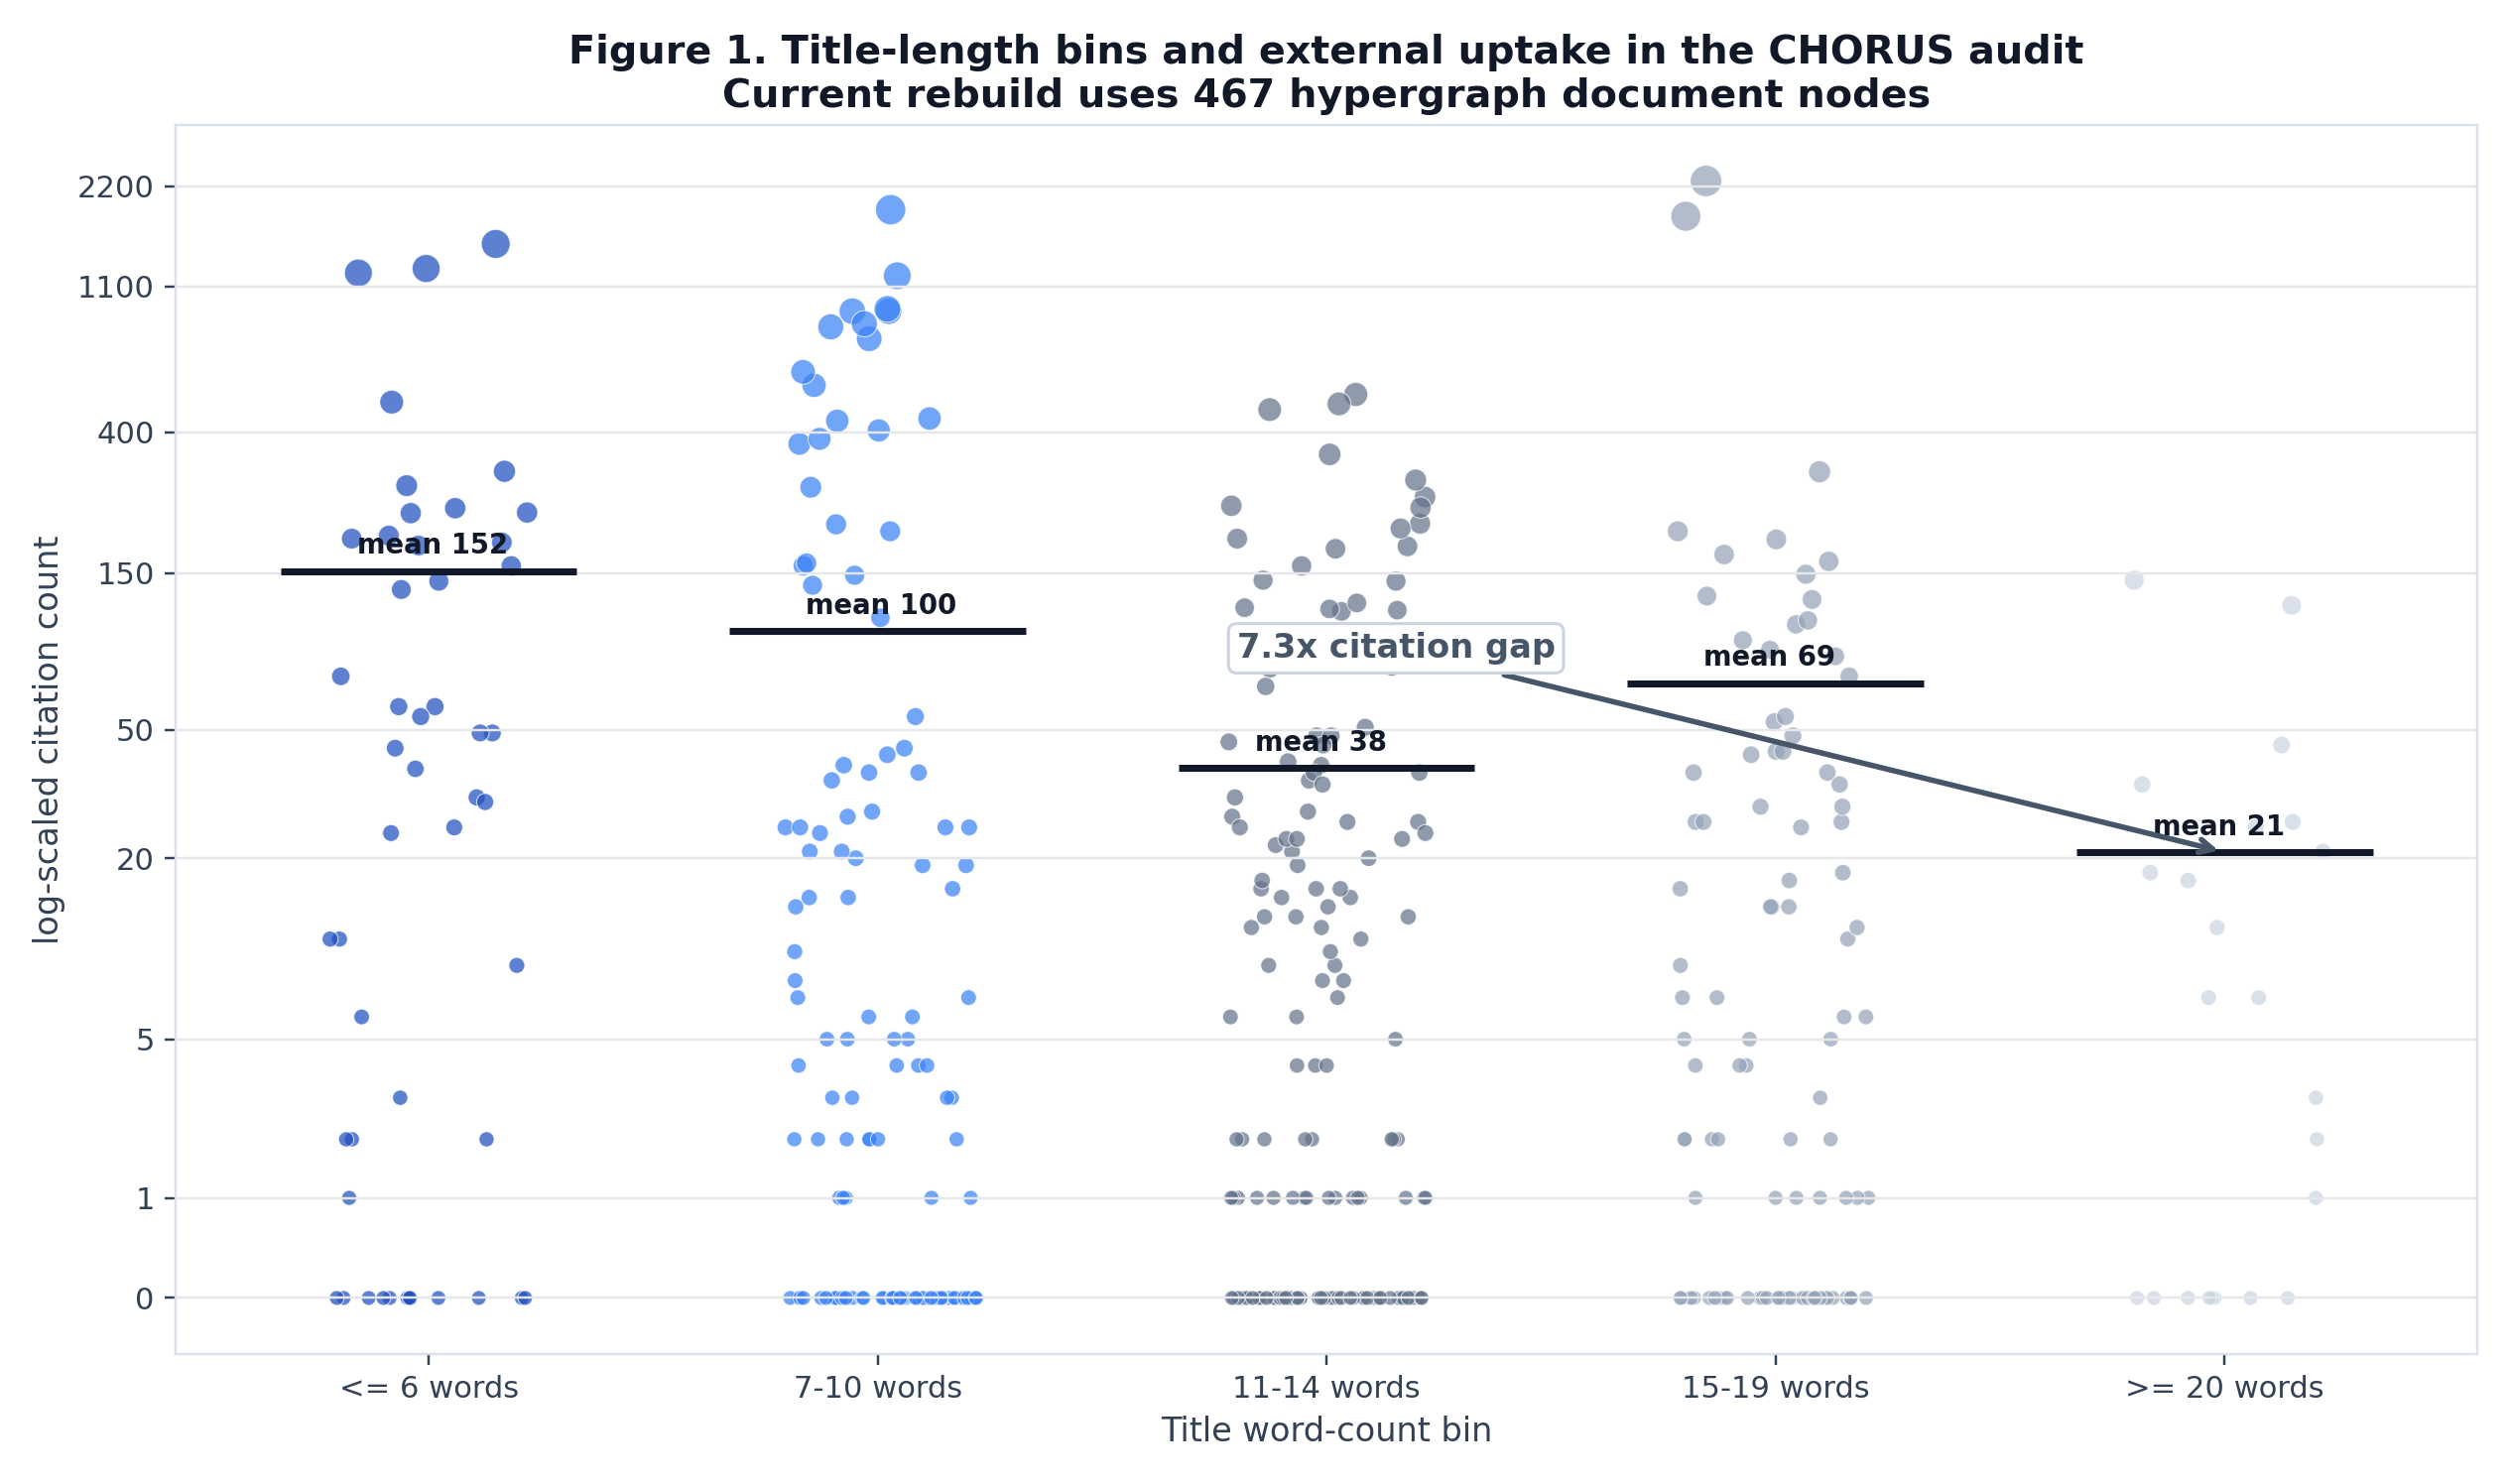
\includegraphics[width=\linewidth]{figure1_title_gradient.png}
\caption{Shorter titles are associated with higher citation impact in the
rebuilt CHORUS sample. Papers with six or fewer title words average 152
citations. Papers with twenty or more words average 21 citations.}
\end{figure}

The first result is deliberately basic. Papers are divided into title word
count bins. If title verbosity were a reasonable stand in for external uptake,
the long title bins should not be sharply worse on a simple impact measure. The
rebuild suggests the opposite. Papers with six or fewer title words average 152
citations. Papers with twenty or more words average 21 citations. The ratio is
7.3 to 1 in favor of the shorter title bin.

This does not mean every short title has stronger influence or every long title
is weak. It also does not mean citations are a complete measure of intellectual
importance.
The interpretation is more precise. A reward signal that uses textual
complexity as a proxy for surprise is exposed to a clear failure mode. It can
reward the form of surprise rather than the substance of surprise. The system
may learn to rank papers that sound unusual, not papers that changed a field or
opened an important research path.

The result also illustrates why proxy audits should begin with simple plots.
The problem is visible before any complex model is introduced. That is useful
for applied research work because teams often need diagnostics that can be
explained, reproduced, and challenged by collaborators who do not work on the
model internals.

\section{Result 2. The Important Papers Are Often Quiet}

\begin{figure}[H]
\centering
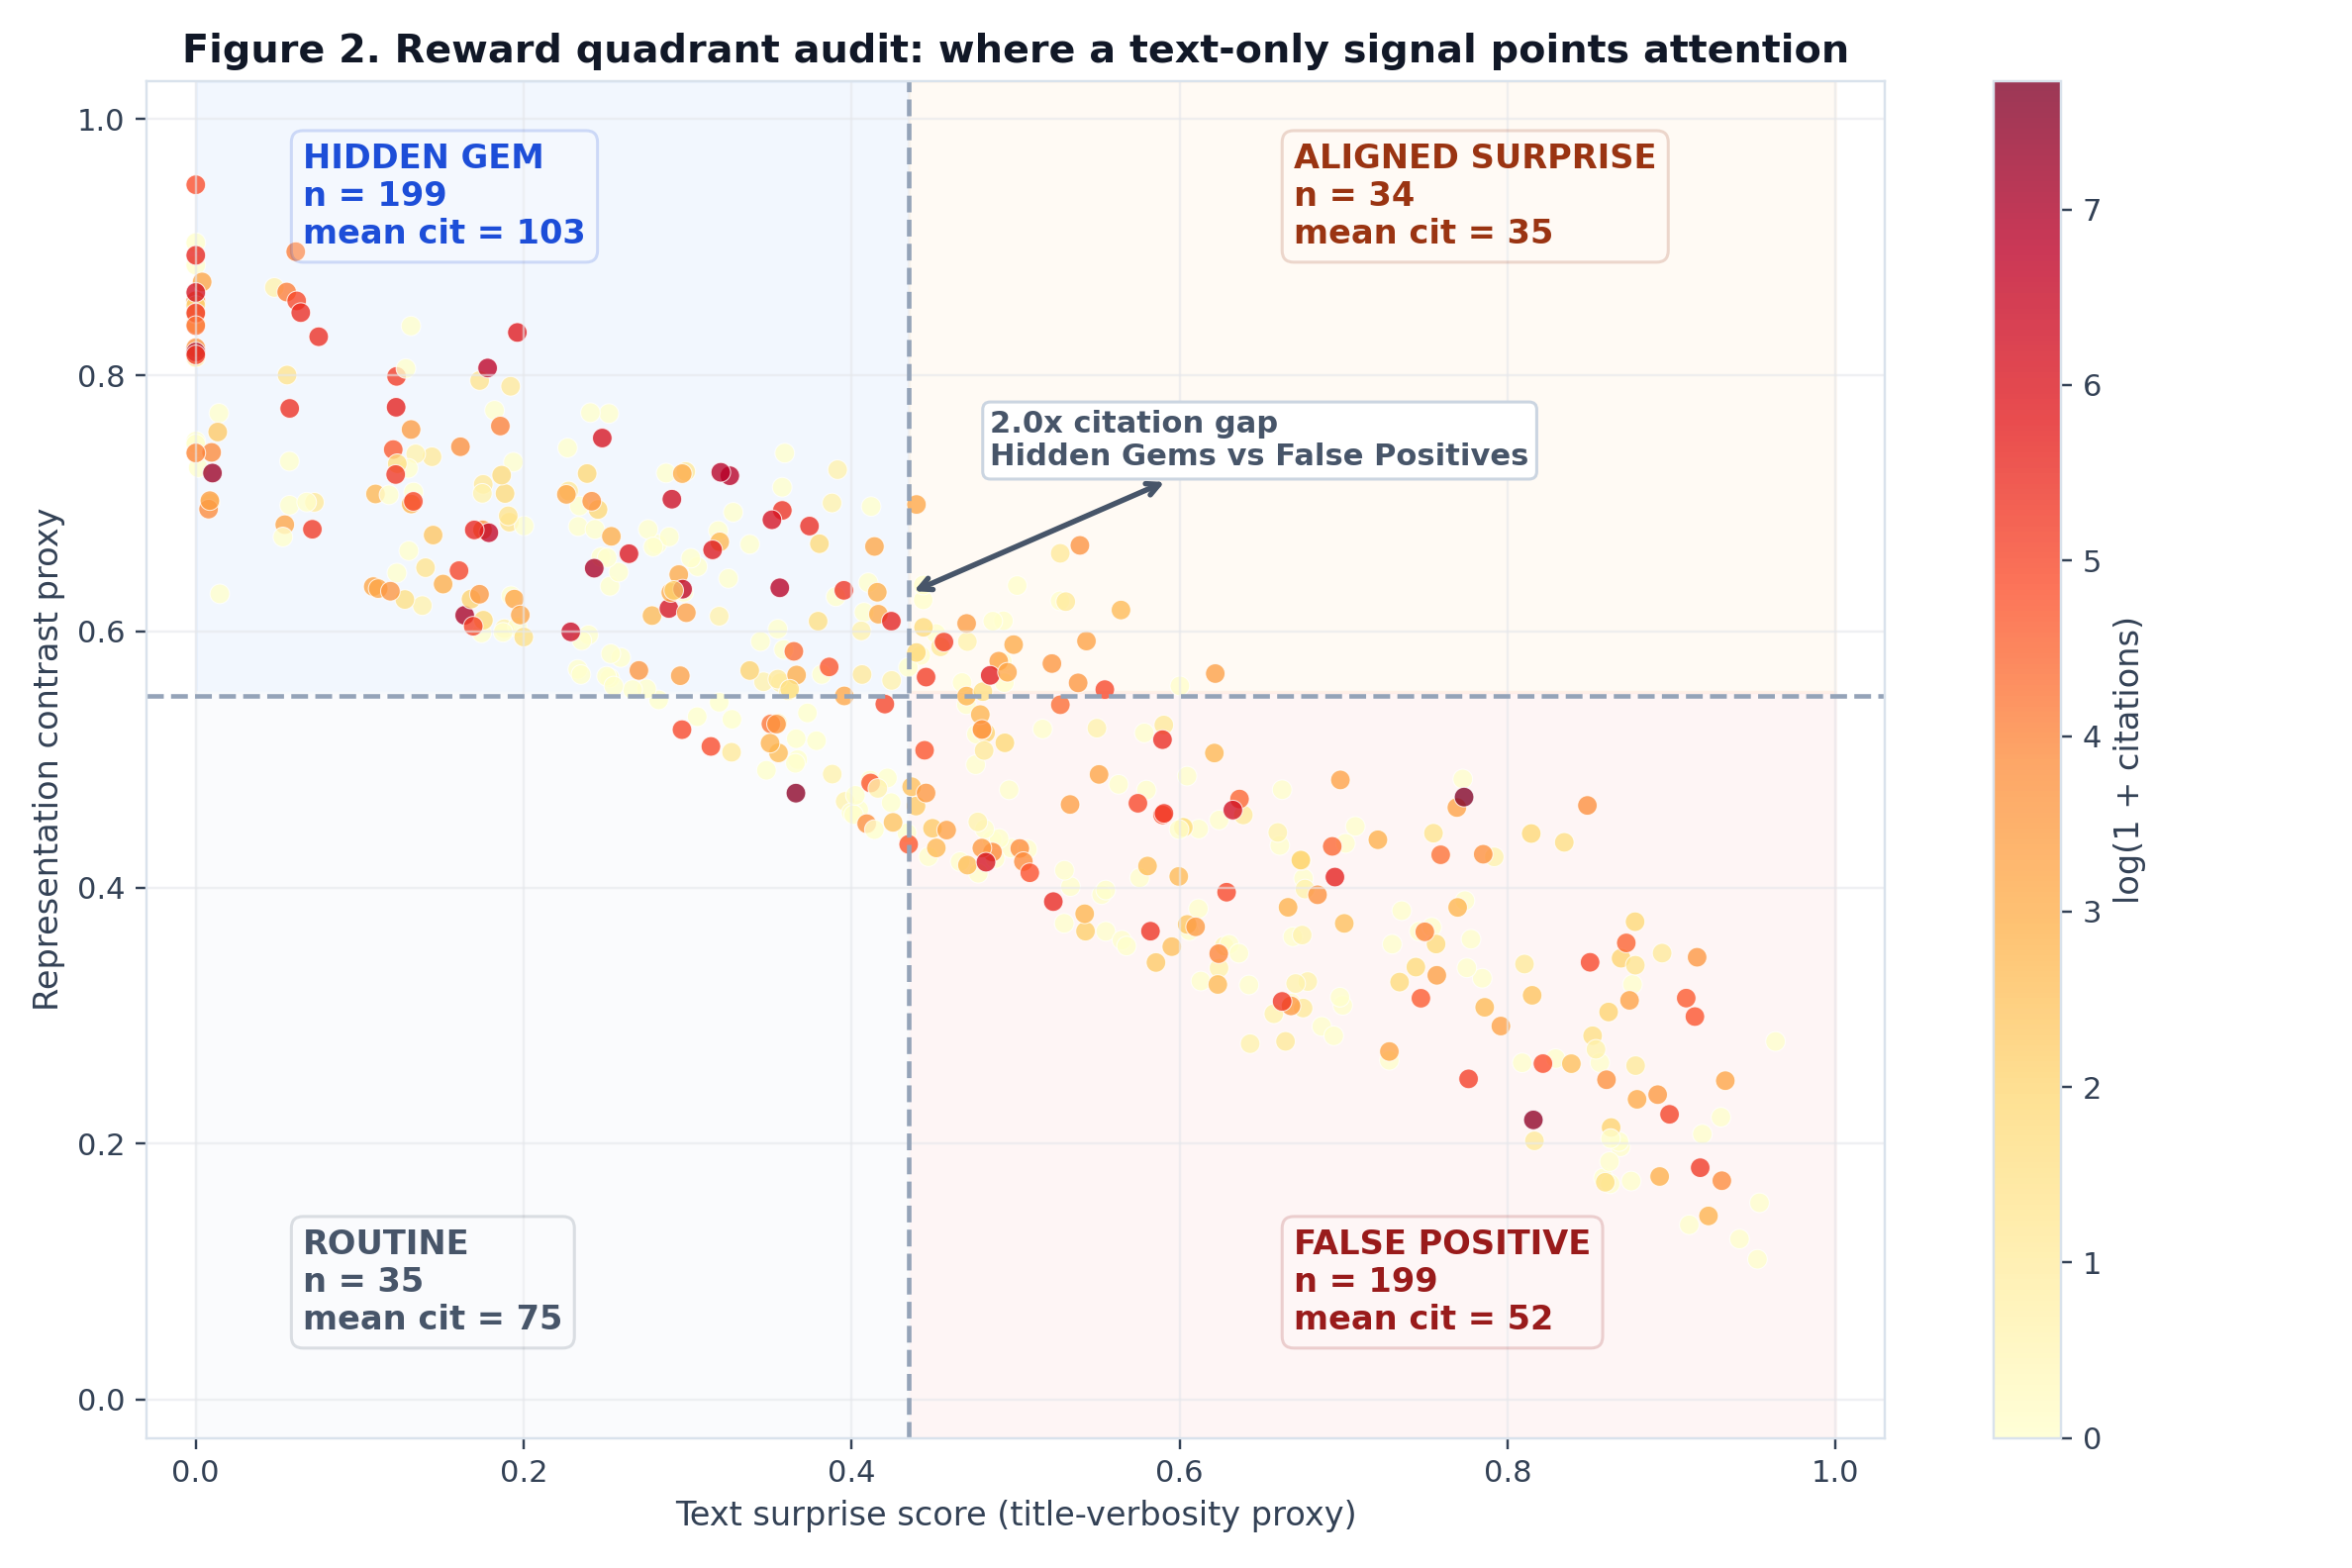
\includegraphics[width=\linewidth]{figure2_reward_quadrants.png}
\caption{The quadrant audit separates quiet high contrast papers from verbose
false positives. Hidden Gems average 97 citations, compared with 43 for False
Positives in the rebuilt sample.}
\end{figure}

The second result places each paper in a two dimensional audit space. The
horizontal axis is the text surprise proxy. The vertical axis is the
representation contrast proxy. The upper left quadrant contains papers that
are quiet in title form but stronger on the contrast proxy. I label these
papers Hidden Gems because they are easy for a title based reward to miss. The
lower right quadrant contains papers that are high on textual surprise but low
on contrast. I label these papers False Positives because they are exactly the
kind of paper a text only reward may over rank.

The citation pattern supports the concern in directional terms. Hidden Gems
average 97 citations. False Positives average 43 citations. The gap is about
2.25 to 1. The result is not a claim that the upper left quadrant is the only
valuable part of the corpus. The routine quadrant also contains influential
papers. The narrower point is that the text heavy, low contrast quadrant looks
weaker on external uptake than the quiet high contrast quadrant. The signal is
therefore shifting attention toward a different region of the research space,
not simply adding random noise.

This matters because ranking systems change what users believe is worth
investigating. A researcher who sees the False Positive quadrant first may spend
time on papers whose titles are elaborate but whose broader signals are weaker.
A founder who receives generic but confident AI advice may spend scarce
resources implementing an action that sounds plausible but does not match the
actual constraint facing the business. In both cases, the failure lives between
the AI output and the human decision.

\section{Result 3. A Role Aware Audit Reveals Who Gets Surfaced}

\begin{figure}[H]
\centering
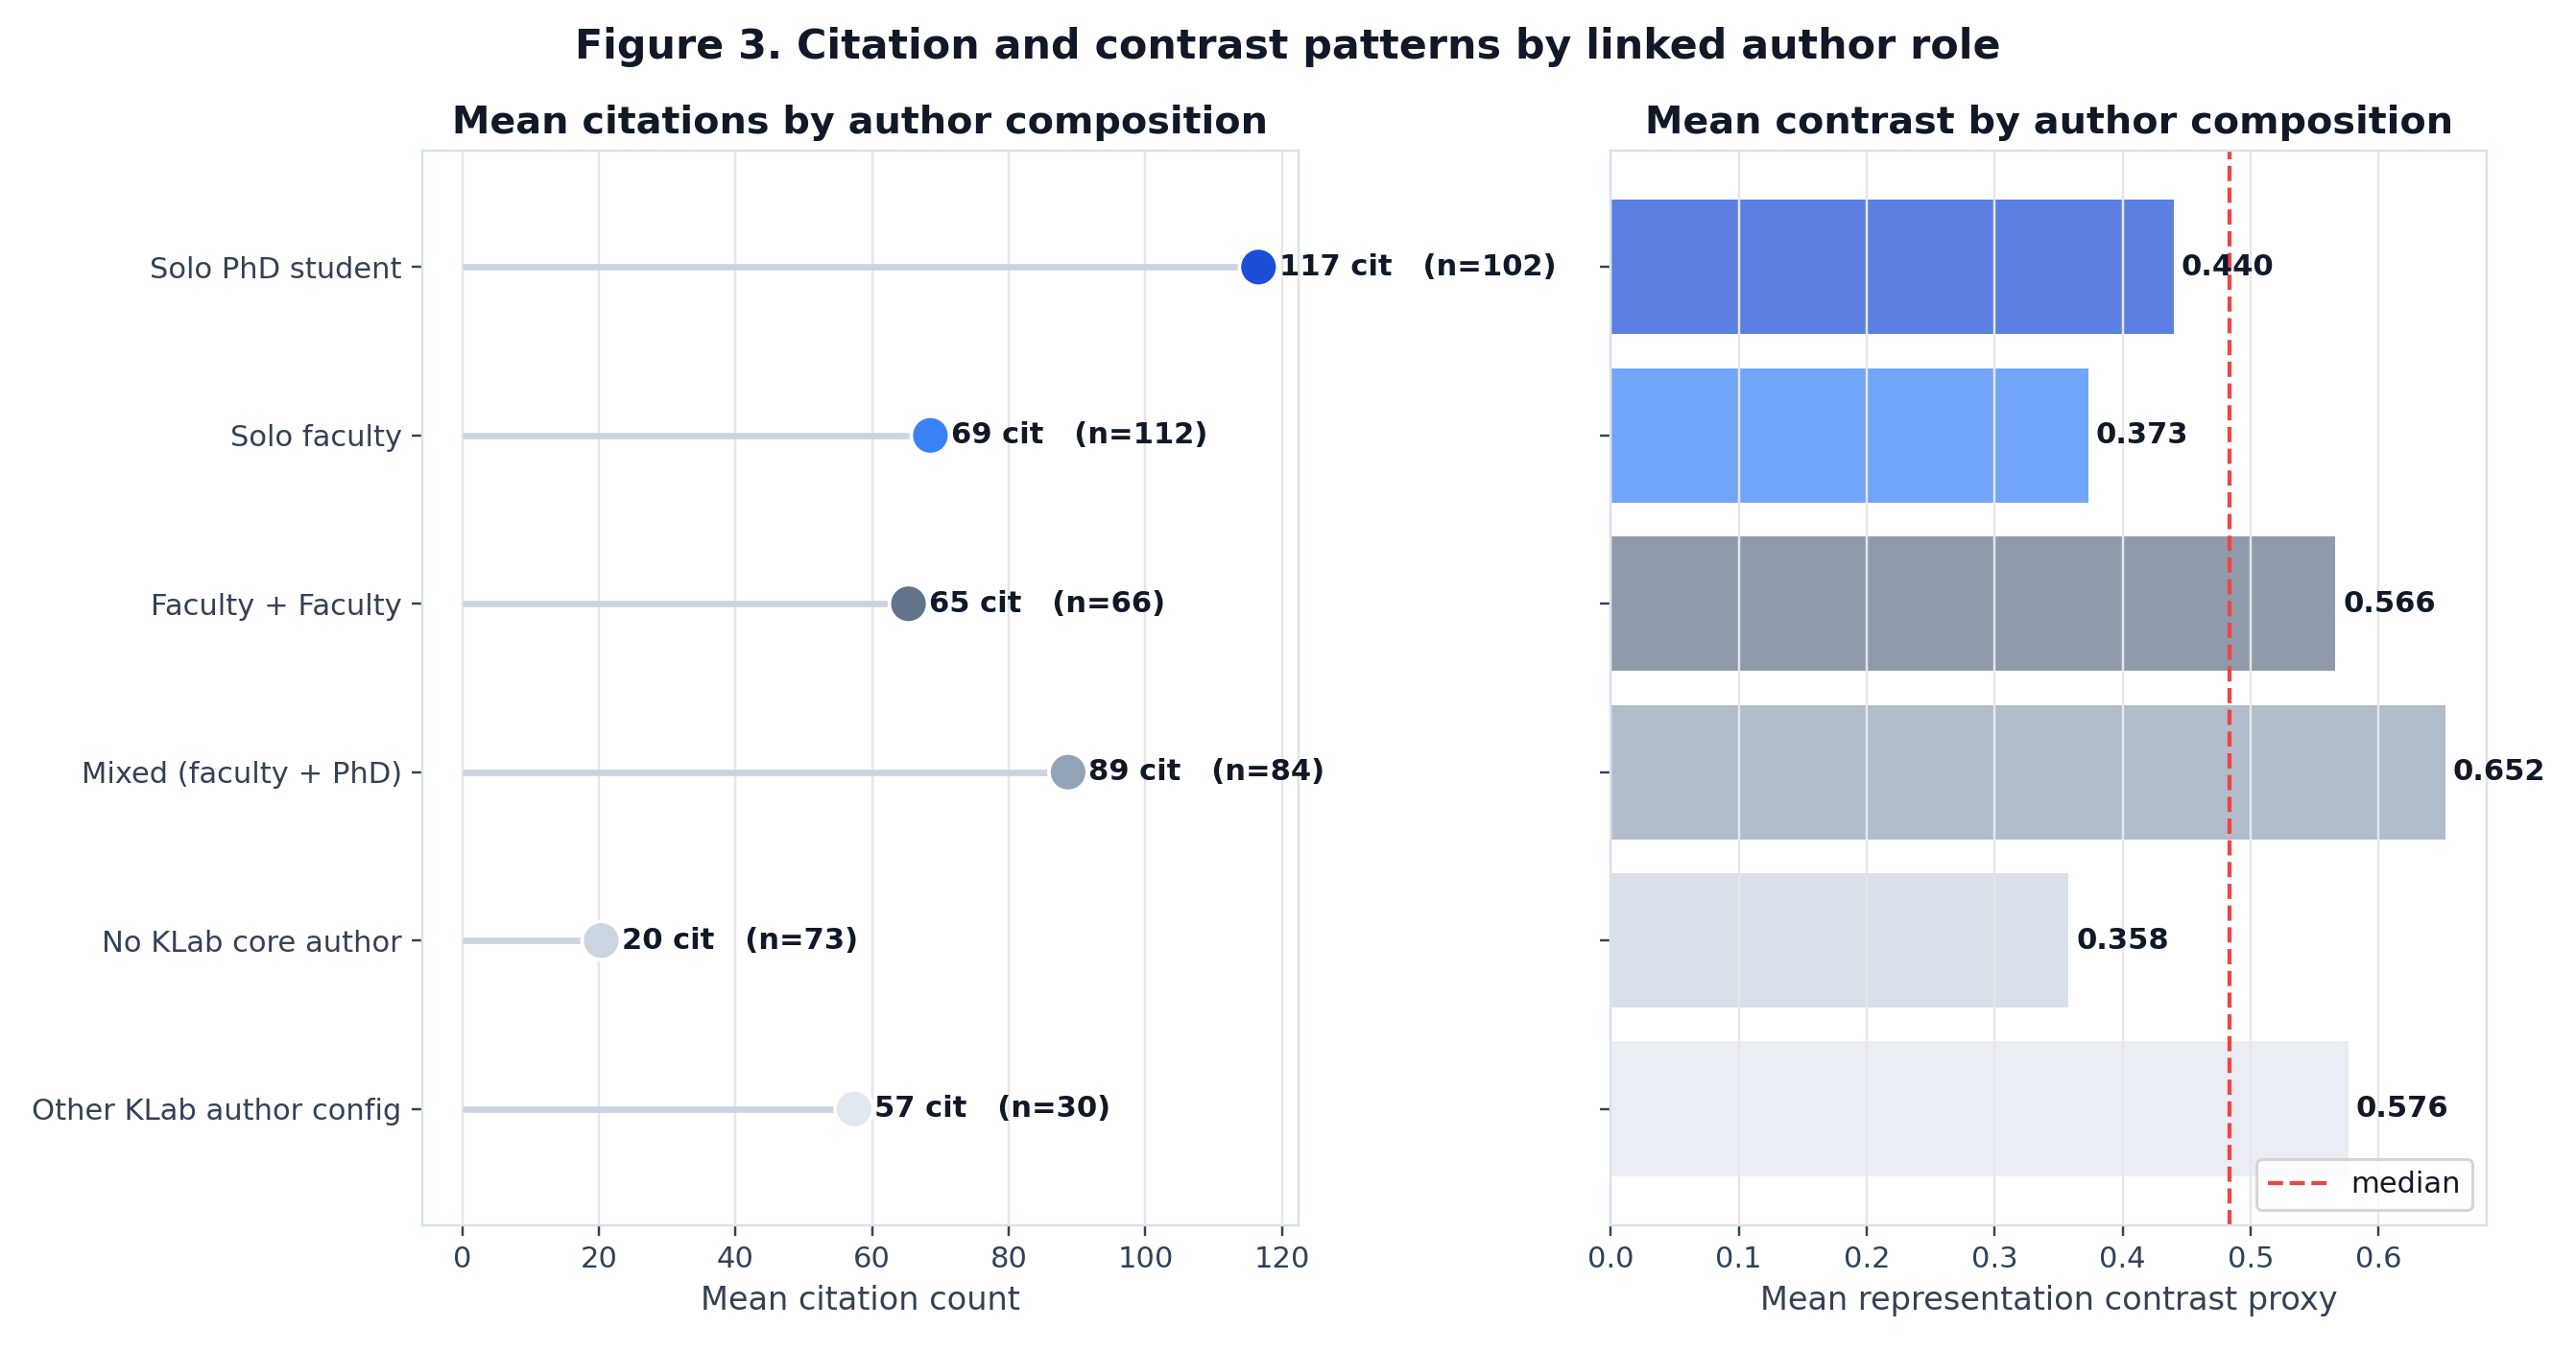
\includegraphics[width=\linewidth]{figure3_author_composition.png}
\caption{A role aware audit checks whether the ranking signal reallocates
attention across author groups. Solo PhD linked papers average 117 citations in
the rebuilt sample, compared with 69 for solo faculty linked papers.}
\end{figure}

The third result asks whether the signal is neutral across author groups. I
group papers by the role composition of their linked authors. The rebuilt sample
suggests that solo PhD linked papers average 117 citations, while solo faculty
linked papers average 69 citations. Mixed faculty and PhD papers average 89
citations. Papers without a core linked author average 20 citations.

This figure should not be read as a claim that student papers are always better
than faculty papers. The data construction is imperfect, and author links come
from a registry rather than from a hand verified authorship file. The useful
point is diagnostic. A reward signal can appear neutral while changing whose
work is visible. If the system ignores role composition, seniority, team type,
or the position of a paper in the lab network, it cannot answer whether its
ranking behavior systematically favors one group of cases.

That diagnostic structure travels well. In an AI advice setting for
entrepreneurs, the equivalent groups might be high performing firms and low
performing firms, experienced founders and first time founders, urban and
non urban firms, or users with different levels of digital fluency. The
question is not whether the AI gives everyone access to text. The question is
whether the AI helps each group select advice that is useful for its actual
decision environment.

\section{Why This Is an Alignment Audit}

The project began from a simple alignment concern. A system can be useful at retrieval while still being poorly aligned in what it chooses to surface. In Russell's language, the problem is not that the system lacks capability. The problem is that a capable system can optimize a misspecified proxy and fail most clearly on the cases where the proxy is least reliable \citep{russell2021human}.

In CHORUS, the convenient proxy is textual surprise. A paper with a long, multi-clause title can look more surprising than a short paper that is central to the lab's research history. That does not mean language-model surprise is useless. Recent work on scientific surprise suggests that perplexity can contain meaningful information about unconventional or transformative research \citep{zhang2025perplexity}. The audit question is therefore more specific: when a text-based surprise signal is used as a ranking proxy, does it still align with external evidence of uptake in this particular corpus?

This is where the representation argument matters. A ranking system may appear to reward intellectual novelty while actually rewarding a surface feature of the text. Work on representation engineering motivates this distinction between what a model appears to express and what its internal or representational signal may be tracking \citep{zou2023representation}. The rebuilt audit keeps that distinction visible by separating a title-based text-surprise proxy from a representation-contrast proxy. This is also why citation counts are held out as an outcome rather than used as an input to the proxy scores.

The current rebuild should be read as a diagnostic audit rather than a final estimate of scientific value. The recovered folder contains 467 hypergraph document nodes, not the earlier 443-paper draft sample. The original perplexity and embedding artifacts were not preserved, so the code reconstructs transparent proxy scores. Under this rebuilt specification, papers with six or fewer title words average 152 citations, while papers with twenty or more title words average 21 citations. Hidden Gem papers average 97 citations, compared with 43 for False Positives. These gaps do not prove that short titles or Hidden Gem status define quality. They show that a text-heavy ranking proxy can direct attention toward a weaker region of the corpus.

This is also a system-level problem rather than only an item-level prediction problem. Work on AI agents argues that AI systems should be evaluated not only by isolated outputs, but by the distribution of cases they make visible and the institutional behavior they induce \citep{gabriel2025ethics,tomasev2025distributional}. In the CHORUS setting, that means asking which papers become salient to users. In other AI advice settings, it would mean asking which recommendations, actions, or opportunities become salient before a human decides.

The role-composition audit follows the same logic. A ranking rule can look neutral while changing whose work is surfaced. In the current rebuild, solo PhD linked papers average 117 citations, while solo faculty linked papers average 69 citations. This should not be interpreted as a claim that student work is generally better than faculty work. The point is that a reward signal should be audited across groups that matter for the institution. Adaptive guardrail work makes a related point: safety checks need to adapt to the agent's environment and history, rather than applying the same static check everywhere \citep{luo2025agrail}. For CHORUS, a role-aware audit is one way to make that environment visible.

The same selection logic can travel to AI advice systems more broadly. A research assistant ranks papers; an AI advisor may rank possible actions; a manager or founder may then choose which suggestion to implement. The key empirical question is not only whether the AI can generate plausible text. It is whether the system helps users select options that fit their actual decision environment. In that sense, CHORUS is a small but concrete example of a broader alignment problem: AI value depends not only on access to generated outputs, but on what the system makes visible, what the user selects, and whether that selected option is actually useful.

\section{What the Code Demonstrates}

The code is designed as a reproducible research artifact rather than a polished
demo. It performs five tasks. First, it reads the raw registry and hypergraph
files. Second, it constructs a paper level panel with visible provenance. Third,
it rebuilds proxy measures while clearly labeling them as proxies. Fourth, it
generates summary statistics and figures from the rebuilt panel. Fifth, it
writes outputs that can be inspected without rerunning the full pipeline.

The most important design choice is transparency. The original model scores
were missing. Instead of filling that gap with opaque assumptions, the code
keeps the missingness visible. It distinguishes raw data from reconstructed
measures and reconstructed measures from outcome variables. That makes the
project easier to criticize and easier to extend. A future version could
replace the title based text surprise proxy with true language model perplexity.
It could replace the contrast proxy with embeddings from abstracts, figures,
or full text. It could also replace citations with downstream measures such as
which papers users choose to read, cite, or connect to new projects.

\section{Limitations}

The audit has three main limitations. First, citation count is an imperfect
outcome. It reflects age, field size, venue, and many forms of visibility that
are not the same as intellectual value. I use it as an external audit signal,
not as the final definition of quality.

Second, the reconstructed scores are proxies. They are useful because they make
the missing code recoverable and the logic inspectable. They are not a
substitute for the original language model and embedding artifacts.

Third, the author composition analysis depends on registry links. Those links
are sufficient for a diagnostic audit, but a publication quality version would
require hand verification of author identities and roles.

These limitations are not incidental. They are part of the research lesson. AI
systems often operate in exactly this kind of data environment: useful but
incomplete, structured but imperfect, rich enough to guide action but risky
enough to require audits. The purpose of the project is to show how I would
turn such a folder into an empirical object with clear assumptions, visible
provenance, and testable claims.

\section{Conclusion}

The CHORUS audit suggests how an AI assistant can create ranking risk even when
it is technically useful. The issue is not that the system cannot retrieve papers. The issue is that a convenient ranking proxy can quietly decide what becomes visible to the user. In the rebuilt data, short titled papers have much higher
average citations than long titled papers, quiet high contrast papers have
higher average citations than verbose false positives, and author role
composition changes how the signal should be interpreted.

The broader implication is that AI advice should be evaluated as a selection system. Access to AI matters, but access alone does not determine value. Value depends on what the AI makes visible, what the user selects, and whether the selected option fits the user's actual environment. The CHORUS case studies this mechanism in a research lab, but the same audit logic can apply to other settings where AI systems rank papers, recommendations, actions, or opportunities before humans decide.

\bibliographystyle{apalike}
\bibliography{references}

\end{document}
